\documentclass[a4paper, 11pt]{scrartcl}

%Packages fuer die Darstellung von Quellcode
\usepackage{beramono} %schoene Schriftart
\usepackage{color}
\usepackage[dvipsnames]{xcolor}
\usepackage{listings}

\usepackage[utf8]{inputenc}
\usepackage[english, ngerman]{babel}
\usepackage[T1]{fontenc}
\usepackage{lmodern}

\usepackage{enumitem}
\usepackage[a4paper, bottom=2cm,includeheadfoot]{geometry}
\usepackage{afterpage} %Um Titelseite mit gesonderter Formatierung zu belegen
\usepackage{blindtext}
\usepackage{todonotes}

% Noetig fuer verschachtelte Imports 
\usepackage{import}
\usepackage{subcaption}

% Bilder
\usepackage{graphicx}

% Header Informationen festgelegt
\usepackage{fancyhdr}
\pagestyle{fancy}
\fancyhf{}
\rhead{\rightmark}
\chead{\thepart}
\lhead{\nouppercase{\leftmark}}
\cfoot{\thepage}


%Quellcodestyle Spezifikationen
\definecolor{DarkPurple}{rgb}{0.4,0.1,0.4}
\definecolor{DarkCyan}{rgb}{0.0,0.5,0.4}
\definecolor{LightLime}{rgb}{0.3,0.5,0.4}
\definecolor{Blue}{rgb}{0.0,0.0,1.0}

% Macro um nicht jedes Mal die listing und namen-Referenz angeben zu muessen
\newcommand{\lstref}[1]{(siehe Listing \ref{#1}, S. \pageref{#1}, \nameref{#1})}


% Syntaxhighlighting festgelegt
\lstdefinestyle{CodeHighlighting} 
{
language=Java, %mit mehreren Sprachen moeglich, ermoeglicht Syntaxhighlighting
columns=flexible,
numbers=left,
frame=single,
frameround=tttt,
showstringspaces=false,
basicstyle=\footnotesize\ttfamily,
keywordstyle=\bfseries\color{DarkPurple},
commentstyle=\itshape\color{LightLime},
stringstyle=\color{Blue}
}

% Titelseite
\title{Entwurfsmuster - von Kopf bis Fuß}
\subtitle{\Large{Zusammenfassung}}
\date{} %Datum unerwuenscht

\newcommand{\prefWidth}{width=0.8\linewidth}

\begin{document}
\newgeometry{a4paper, bottom=5cm}
\maketitle
\pagestyle{plain}
\tableofcontents
\clearpage
\pagestyle{fancy}

\section{Entwurfsprinzipien}
Essenz jedes Musters kurz zusammengefasst. 

\begin{itemize}[leftmargin=0.2in]
	\item Entwurfsprinzipien:
	\item Identifizieren Sie die Aspekte Ihrer Anwendung, die sich aendern koennen und trennen Sie sie 
  von denen, die konstant bleiben.
	\item Programmieren Sie auf eine Schnittstelle, nicht auf eine Implementierung.
	\item Ziehen Sie die Komposition der Vererbung vor.
	\item Streben Sie bei Entwuerfen mit interargierenden Objekten nach lockerer Kopplung (einfachere 
Erweiterung moeglich).
	\item Klassen sollten fuer Erweiterung offen, aber fuer Veraenderung geschlossen sein. (Mit Vorsicht zu 
betrachten, dies fuehrt zu hoeherer Komplexitaet und sollte nur in sinnvollen Faellen 
angewendet werden.)
	\item Stuetzen Sie sich auf Abstraktionen. Stuetzen Sie sich nicht auf konkrete Klassen.  
\end{itemize}

	



\clearpage
\section{Strategy-Muster}

\subsection{Problemstellung}
\begin{itemize}
\item Es soll eine Simulation fuer ein Spiel mit diversen Entenarten geschrieben werden.
\item Entenarten besitzen verschiedene Eigenschaften.
\item In manchen Faellen nicht nur verschiedene Auspraegungen, sondern sogar nicht existent. 
\item Verschiedene Arten sollen aber alle von der selben Klasse erben. 
\end{itemize}

\subsection{L"osung}
Problem hierbei (Lsg.): 
Wenn  dies direkt in die Klasse geschrieben  wird ist diese sehr schlecht wartbar,  denn die Klassen selbst 
sind  sehr  schlecht wartbar. Die  Loesung  hierbei,  das  Strategy-Muster.  Man versucht  aehnliche
Algrothmen wie z.B. das Flug- oder Quakverhalten in eine Gruppe/Familie von Algorithmen 
zusammenzufassen (zu kapseln). Dies geschieht mithilfe verschiedener Interfaces z.B. 
Quakverhalten  /  Flugverhalten.  Die  Mutterklasse  besitzt  entsprechende  Felder  von  den  Typen
Quak-/Flugverhalten.  Diese werden entsprechend gesetzt  und in  den jeweiligen Methoden aufgerufen.
Die  aufrufenden erbenden  Klassen implementieren  das  entsprechende  Interface und  koennen so das
gewuenschte Verhalten  implementieren.  Hierbei  gestaltet  sich  die  Wartung  des  Codes  deutlich
einfacher.

\subsection{Erkl"arung des Musters}
\paragraph{Definition}
Das  Strategy-Muster definiert  eine  Familie von Algorithmen,  kapselt  sie  einzeln  und macht sie
austauschbar. Das Strategy-Muster  ermoeglicht  es, den  Algrithmus unabhaengig  von den Clients die
ihn einsetzen, variieren zu lassen.

\paragraph{Vorteile}
Bei  diesem  Entwurft  koennen  andere Typen  von  Objekten unsere  Flug- und  Quakverhalten  wieder
verwenden (Bezug zu Kap. 1), weil diese Verhalten nicht mehr in unseren Ente-Klassen verborgen sind.
Wir  koennen  neue Verhalten hinzufuegen, ohne  irgendeine unserer bestehenden  Verhaltensklassen zu
aendern oder Hand an eine der Enten-Klassen zu legen, die Flugverhalten nutzen. 

\begin{figure}
	\centering
	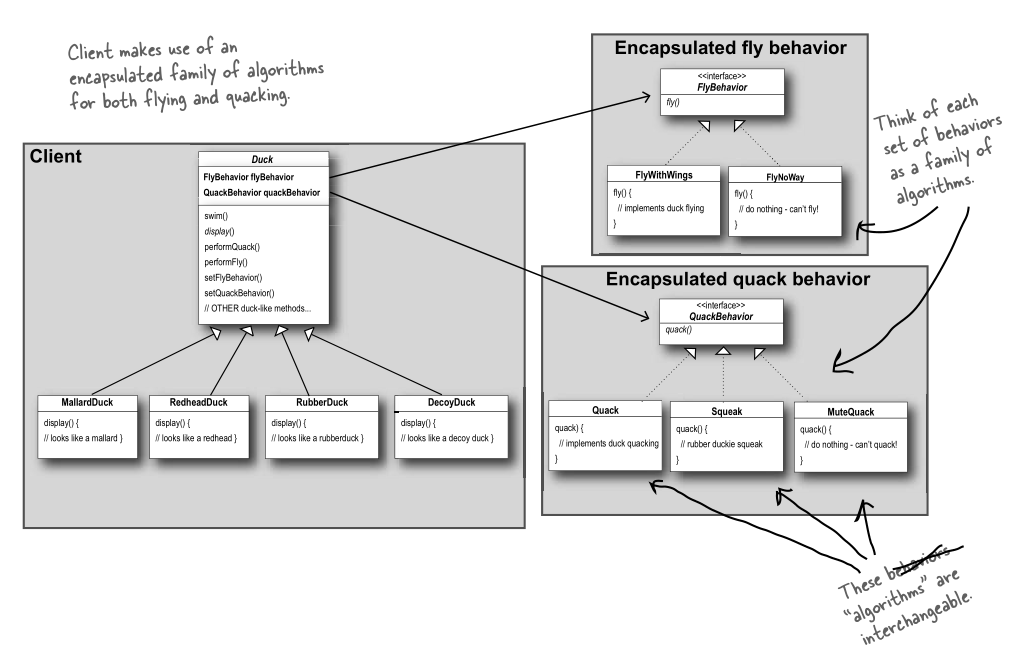
\includegraphics[width=\linewidth]{strategy/img/strategyUML}
	\caption{UML-Darstellung des Strategy-Musters}
	\label{fig:strategyUML}
\end{figure}
\clearpage
\section{Decorator-Muster}

\subsection{Problemstellung}
\begin{itemize}
\item Ein B"acker m"ochte verschiedene Kaffeesorten verkaufen. 
\item Es soll m"oglich sein verschiedene Bonuszutaten (z.B. Sahne, Zucker, etc.) hinzuzuf"ugen. 
\item Hierbei kann die Menge der variieren. Es ist also m"oglich sowohl eine Extra-Portion, als auch 
  zwei extra Portionen Sahne dazu zu bestellen. 
\item Ausserdem ist es m"oglich verschiedene Zutaten zu kombinieren. 
\item Problem: Wenn man sich auf einfache Vererbung beschr"ankt wird die Stuktur sehr schnell 
  un"ubersichtlich. 
\end{itemize}

\subsection{L"osung}
Es wird zu allererst eine abstrakte Klasse Getr"ank gebildet, von der sowohl die Zutaten als auch 
die Kaffeesorten erben. Die Kaffesorten tun dies direkt. Sie besitzen zwei Felder f"ur die 
Beschreibung und den Preis, "uber entsprechende Getter sind sie abrufbar. Nun bildet man eine 
abstrakte Wrapper-Klasse von der s"amtliche Zutaten erben sollen. Jede Zutat erbt von der Wrapper 
Klasse und muss die Getter f"ur die Beschreibung / Preis neu implementieren, denn jede Zutat 
h"alt eine Referenz auf ein Getr"ank welches im Konstruktor gesetzt wird. Bei den Gettern wird 
die Beschreibung / Preis an die Werte des Getr"anks angeh"angt bzw. drauf addiert. Da alle 
Klassen von der selben Superklasse ableiten kann die Referenz nicht nur einen Kaffee ohne Zutaten 
sondern auch einen mit diesen beinhalten. Die Wrapper-Klasse ist letztendlich dazu da eine 
Schnittstelle herzustellen, damit es sowohl geordnet ist und die Referenz wie erw"ahnt 
bereits modifizierte Objekte halten kann. 

Beim Bestellen wird eine zugrunde liegende Kaffesorte gew"ahlt (z.B. Espresso). Diese wird mit 
den einzelnen Zutaten "dekoriert" (Bsp. siehe main Klasse im Code). 

\subsection{Erkl"arung des Musters}
\paragraph{Definition}
Decorator - F"ugt einem Objekt dynamisch zus"atzliche Verantwortlichkeit hinzu. Dekorierer bieten 
eine flexible Alterntive zur Ableitung von Unterklassen zum Zweck der Erweiterung der 
Funktionalit"at.

\paragraph{Punkt f"ur Punkt (S.105)}
\begin{itemize}
\item Vererbung ist eine Form von Erweiterung, aber nicht notwendigerweise der beste Weg, um Ihren 
  Entw"urfen Flexiblit"at zu verleihen. 
\item Unsere Entw"urfe sollen die Erweiterung von Verhalten ermoeglichen, ohna dass dazu bestehnder 
  Code ge"andert werden m"usste.
\item Oft keonnen Komposition und Delegierung verwendet werden, um zur Laufzeit neue Verhalten 
  hinzuzuf"ugen.
\item F"ur die Erweiterung von Verhalten bietet das Decorator-Muster eine Alternative zur Ableitung 
  von Unterklassen.
\item Das Decorator-Muster schliesst einen Satz von Dekorierer-Klassen ein, die verwendet werden, um 
  konkrete Komponenten einzupacken. 
\item Dekorierer-Klassen spiegeln den Typ der Komponente wider, die sie dekorieren. (Sie haben sogar 
  tats"achlich den gleichen Typ wie die Komponente, die sie dekorieren, entweder durch Vererbung 
  oder durch die Implementerung eines Interface.)
\item Dekorierer "andern das Verhalten der Komponenten, indem sie vor und / oder nach (oder auch an 
  Stellen von) Methodenaufrufen auf der Komponente neue Funktionalit"aten hinzuf"ugen. 
\item Sie koennen eine Komponente mit einer bliebigen Zahl vn Dekorierern einpacken. 
\item Dekorierer sind f"ur die Clients der Komponente "ublichweise transparent, ausser wenn sich der 
  Client auf den konkreten Typ der Komponente st"utzt.
\item Dekorierer koennen in Ihren Entw"urfen zu vielen kleinen Objekten f"urhen, und eine 
  "uberm"assige Verwendung kann den un"ubersichtlich machen.  
\end{itemize}
 
\paragraph{Wann das Decorator-Muster ungeeignet ist}
\begin{itemize}
\item Wenn Sie mit Code arbeiten, der auf den Typ einer konkreten Komponente angewiesen ist, 
  zerbrechen Dekorierer diesen Code. Solange Sie nur Code auf Basis des abstrakten 
  Komponententyps schreiben, bleibt die Verwendung von Dekorierern f"ur ihren Code transparent.
  (Muster z.B. f"ur Rabatsystem beim Kaffeehaus aus diesem Kapitel ungeeignet.)
\item Dekorierer sollen den Objekten, die sie einpacken Verhalten hinzuf"ugen. Wenn Sie begninnen, 
  auf mehreren Schichten in der Dekoriererkette zu blicken, dann strecken Sie Decorator "uber 
  seinen eigentlichen Zweck.
\end{itemize}
  
\paragraph{Gut zu wissen}
\begin{itemize}
\item Die java.io-Klassen verwenden ebenfalls das Decorator-Muster. Es gibt diverse Streams mit 
  jeweils unterschiedlichen Aufgaben, und es gibt die Klasse FilterInputStream die als Superklasse 
  f"ur verschiedene Dekorierer arbeitet.
\end{itemize}

\begin{figure}
	\centering
	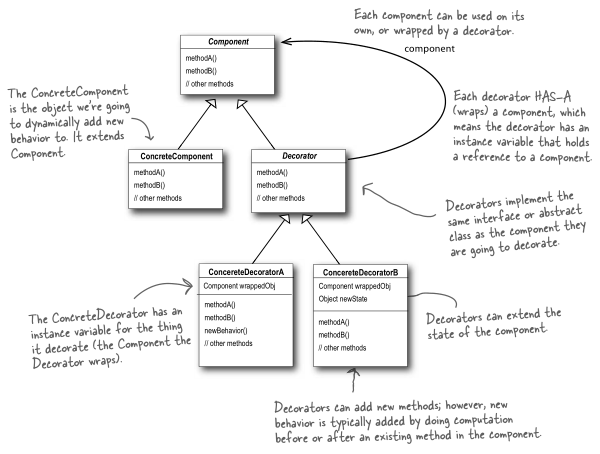
\includegraphics{decorator/img/decoratorUML}
	\caption{UML-Darstellung des Decorator-Musters}
	\label{fig:decoratorUML}
\end{figure}

\clearpage
\section{Observer-Muster}
\subsection{Problemstellung}
\begin{itemize}
	\item Wetterstation liefert Daten (Luftdruck, Temperatur, etc.).
	\item Gefragt ist ein WetterDaten-Objekt. 
	\item Diverse Anzeigeger"ate sollen in der Lage sein, sich die Daten vom WetterDaten-Objekt zu ziehen 
und entsprechend darzustellen. Problematisch wird es, wenn verschiedene Anzeigeger"ate nur 
bestimmte Daten anzeigen sollen. 
	\item Besonderes Augenmerk bei dieser Aufgabe, die Daten sollen mit einem einzigen Aufruf 
aktualisiert werden. 
	\item Wichtig: Es soll m"oglich sein neue Anzeiger"ate einzubinden. Hierbei soll der zus. Aufwand so 
gering wie m"oglich gehalten werden. 
\end{itemize}

\subsection{L"osung}
\paragraph{Muster (Grunds"atzliches Prinzip):}
Man definiert ein Interface z.B. \enquote{Subjekt} das die Schnittstelle f"ur das WetterDaten-Objekt 
angibt. Hierzu geh"oren die Methoden um einen Beobachter zu registrieren, zu entfernen oder 
diesen "uber die Aktualisierung der Daten zu informieren (bzw. ihm diese zukommen zu lassen). Die 
Idee beim Observer-Muster ist n"amlich, dass ein Datenobjekt mit entsprechenden Feldern ein 
Attribut mit einer Liste von Beobachtern h"alt die Zugriff auf die Felder besitzen. Dies kann 
mithilfe einer "Ubergabe des Objektes geschehen oder aber mit einer tats"achlichen "Ubergabe von 
Parametern. Mit den Methoden zum Registrieren und Entfernen werden die Beobachter der Liste 
hinzugef"ugt oder entfernt. Das WetterDaten-Objekt aus dem Bsp. implementiert jetzt dieses 
Interface. Anschliessend wird ein zweites Interface f"ur die Beobachter (im Bsp. die 
verschiedenen Anzeige-Klassen) geschrieben. Die Beobachter informieren dieses jeweils und haben 
damit Zugriff auf eine Methode zum Aktualisieren der Werte. Hier k"onnen direkt die Parameter 
"ubergeben werden, oder aber das Datenobjekt selbst (um mit Gettern die Daten zu "ubermitteln). 

\paragraph{Muster aus java.util.Observable / Observer}
Es gibt bereits ein vorgefertigtes Observer-Muster in der Standardbibliothek \emph{util}. Hier erbt das 
jeweilige Datenobjekt von der Superklasse Observable. Diese Klasse bringt bereits die Liste aus 
Beobachtern und weitere Methoden wie die setChanged() und notfyObservers() Methoden. Wichtig 
hierbei ist zu beachten, dass man erst die Beobachter benachrichtigen kann wenn setChanged 
aktiviert wurde. NotifyObservers() ist ausserdem "uberladen, denn es ist ist m"oglich neben dem 
eigentlichen Datenobjekt (hier WetterDaten-Objekt) noch ein anderes zu "ubergeben, welches z.B. 
weitere Werte enthalten kann. 
Zum genauen Aufbau siehe Code.

\begin{samepage}
\paragraph{Nachteile der Standardbibliothek}
\begin{itemize}
\item Reihenfolge der Auswertung "andert sich -> Ungeeignet f"ur Anwendungen wo dies von Bedeutung 
  sein sollte.
\item Observable ist eine Klasse und kein Interface -> Klasse kann daher keine andere Klasse 
  erweitern und schlecht wartbar sowie wiederverwendbar.
\item Observable sch"utzt entscheidende Methoden -> z.B. setChanged(), kann daher auch nur von 
  erbenden Klassen aufgerufen werden.
\end{itemize}
\end{samepage}

\subsection{Erkl"arung des Musters}
\paragraph{Definition}
Das Observer-Muster definiert eine Eins-zu-viele-Abh"angigkeit zwischen Objekten in der Art, dass 
alle abh"angigen Objekte benachrichtigt werden, wenn sich der Zustand des einen Objekts "andert. 

\paragraph{Gutes Alltagsbeispiel} 
Zeitungsabonnementsdienst
\begin{itemize}
\item Man m"ochte Abonnent werden -> man wird auf die Liste der Abonennten gesetzt. 
\item Neue Ausgabe wird ausgegeben (aktualisiert) -> Alle Abonnementen der Liste werden benachrichtigt. 
\item Bei der Standardbibliothek \emph{utils} ist bereits ein solches Muster vorgegeben mit dem es f"ur die 
  Abonennten sogar m"oglich ist sich jederzeit per Getter-Methoden die Daten zu ziehen ohne das 
  eine entsprechende Methode im Subjekt aufgerufen werden muss.
\item Auf Wunsch ist es ebenfalls m"oglich wieder aus der Liste der Abonennten auszutreten. 
\end{itemize}

\paragraph{Punkt f"ur Punkt Zusammenfassung (S. 74)}
\begin{itemize}
\item Das Observer-Musster definiert ein Eins-zu-viele-Verh"altnis zwischen Objekten.
\item Subjekte oder, wie wir sie auch kennen, Observables aktualisieren Beobachter "uber eine 
  Schnittstelle.
\item Die Beobachter sind insofern locker angebunden, als das Observable "uber sie nichts anderes 
  wei"s, als dass sie das Interface Observer implementiern. 
\item Sie k"onnen Daten aus dem Observable herausgeben oder herausziehen, wenn Sie das Muster 
  verwenden (wobei das Herausziehen als die \enquote{richtigere} Methode betrachtet wird). 
\item Verlassen Sie sich nicht auf eine bestimmte Reihenfolge der Benachrichtigung Ihrer Beobachter. 
\item Java besitzt eine Reihe von Implementierungen des Observer-Musters, einschlie"slich des 
  allgemeinen java.util.Observable.
\item Nehmen Sie sich vor den Haken der Implementierung von java.util.Observable in Acht. (Siehe 
  Erkl"arung Kap. 1).
\item Haben Sie keine Hemmungen, Ihre eigene Observable-Implementierung zu schreiben, wenn dies 
  erforderlich ist.
\item Swing macht wie andere GUI-Frameworks extensiven Gebrauch vom Observer-Muster.
\item Sie finden das Muster auch an vielen anderen Orteien einschliesslich JavaBeans und RMI. 
\end{itemize}

\subsection{Aufgabe zu den Entwurfsprinzipien}
\paragraph{Aufgabe zu den Entwurfsprinzipien}
Beschreiben Sie f"ur jedes Entwurfsprinzip, wie das Observer-Muster das Prinzip umsetzt. 

\paragraph{Prinzipien}
\begin{enumerate}
\item Identifizieren Sie die Aspekte Ihrer Anwendung, die sich "andern k"onnen und trennen Sie sie 
   von denen, die konstant bleiben.
\item Programmieren Sie auf eine Schnittstelle, nicht auf eine Implementierung.
\item Ziehen Sie die Komposition der Vererbung vor.
\end{enumerate}

\paragraph{Eigene Erkl"arung}
\begin{enumerate}
\item Beobachter k"onnen sich "andern, werden daher zusammengefasst und ausgelagert.
\item Da die Beobachter lediglich ein Interface implementieren und keine Klasse erweitern, besteht 
   hier eine lose Bindung d.h. man Programmiert auf eine Schnittstelle.
\item Die beiden Parteien (Beobachter, Subjekt) implementieren jeweils nur ein Interface und 
   erweitern keine Superklasse.
\end{enumerate}
   
\paragraph{Erkl"arungen aus dem Buch (S. 77)}
\begin{enumerate}
\item Das, was beim Observer-Muster variiert, ist der Zustand des Objekts und die Anzahl sowie die 
   Typen der Beobachter. Mit diesem Muster k"onnen Sie die Objekte variieren, die vom Zustand des 
   Objekts abh"angig sind, ohne das Subjekt ver"andern zu m"ussen. Das nennt man verausschauend 
   handeln!
\item Subjekt und Beobachter nutzen beide Interfaces. Das Subjekt h"alt Objekte nach, die das 
   Interface Observer implementieren, w"ahrend die Beobachter sich registrieren und vom 
   Subjekt-Interface benachrichtigt werden. Wie wir gesehen haben, h"alt das die Dinge 
   ordentlich und locker gebunden. 
\item Das Observer-Muster nutzt Komposition um eine beliebige Anzahl von Beobachtern mit ihren 
   Subjekten zu verbinden. Diese Beziehungen werden nicht durch irgendeine Art von 
   Vererbungshierarchie implementiert. Nein sie werden zur Laufzeit durch Komposition eingerichtet!
\end{enumerate}

\FloatBarrier
\begin{figure}[b!]
	\centering
	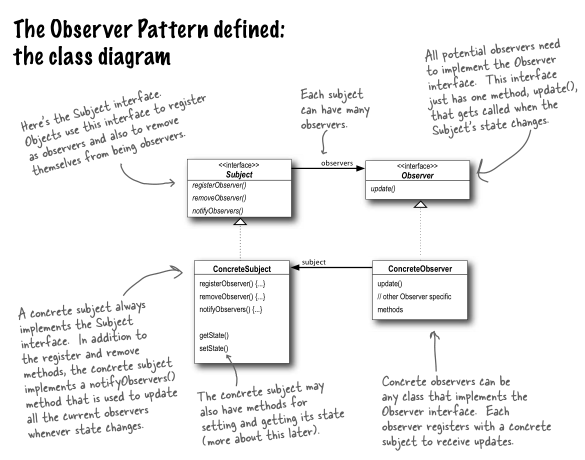
\includegraphics[width=\linewidth]{observer/img/observerUML}
	\caption{UML-Darstellung des Observer-Musters}
	\label{fig:observerUML}
\end{figure}

\clearpage
\section{Singleton-Muster}
\subsection{Definition}
Das Singleton-Muster sicher, dass es nur eine Instanz einer Klasse gibt, und bietet einen globalen 
Zugriffspunkt fuer diese Instanz. 

\subsection{Erklaerung}
\begin{itemize}
\item Wir nehmen eine Klasse und lassen sie eine einzige Instanz von sich selbst verwalten. Wir 
  verhindern auch, dass irgendeine andere Klasse eigenstaendig eine neue Instanz erstellt. Um eine 
  Instanz zu erhalten, muss man ueber die Klasse selbst gehen. 
\item Wir bieten ausserdem einen globalen Zugriffspunkt fuer die Instanz: Jedes Mal wenn Sie eine 
  Instanz benoetigen, fragen Sie einfach be der Klasse nach, und diese reicht Ihnen, die eine 
  Instanz. Wie Sie gesehen haben, koennen wir das so implementieren, dass das Singleton verzoegert 
  erstellt werden kann, was bei ressourcenintensiven Objekten besonders wichtig ist. 
\end{itemize}

\FloatBarrier

\begin{figure}
	\centering
	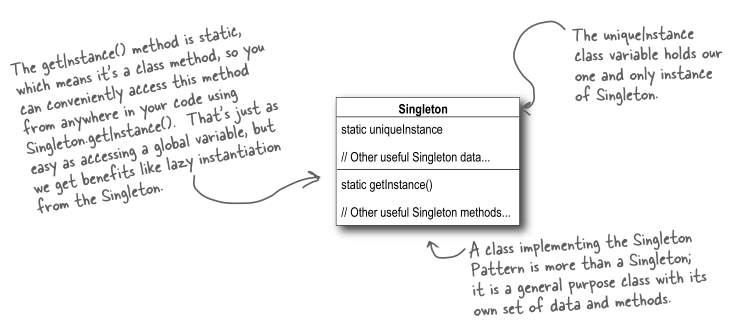
\includegraphics[width=.8\linewidth]{singleton/img/singletonUML}
	\caption{UML-Darstellung des \emph{einfachen} Singleton-Musters}
	\label{fig:singletonUML}
\end{figure}
\clearpage
\section{Factory-Muster}
\subsection{Problemstellung} Einfach
\begin{itemize}
\item Man moechte eine Pizzeria mit mehreren Zweigstellen erstellen.
\item Bei der Zubereitung der Pizza gibt diverse Arbeitsablaeufe die von den Zweigstellen allesamt 
  unterschiedliche abgearbeitet werden koennen (Z.B. Schneiden: Vierteln vs. in acht Stuecke 
  schneiden, etc.).
\item` Problem: Um Code-Dopplung zu vermeiden sollen die Pizza in einer einzigen Klasse implementiert 
  sein -> Es muss ein Pizza-Objekt entsprechend den Anforderungen (welche Zweigstelle?) erstellt 
  werden. 
\end{itemize}
  
\subsection{Loesung}
Es wird eine abstrakte Superklasse \emph{Pizzeria} erstellt. Verschiedene Zweigstellen beerben diese. 
Jede dieser Zweigstellen implementiert eine Methode \emph{erstellePizza()}. Diese dient als so 
genannte Factory, denn sie erstellt ein Objekt des gew"unschten Typs. Bei der Erstellung wird ein 
entsprechender Konstruktor einer speziellen Pizza-Klasse aufgerufen. Diese Klasse implementiert 
die Methoden der Arbeitsschritte (backen, schneiden, etc.) entsprechend. In der Superklasse wird 
eine Methode deklariert ("bestellePizza()") die mit diesem Objekt arbeitet. Durch den 
Polymorphismus / Abstraktion ist es irrelevant mit welchem Pizza-Objekt man arbeitet, da alle 
erbenden Klassen des Pizza-Typs die dort aufgerufenen Methoden implementiert / geerbt haben. Die 
Methode "bestellePizza()" wird auch fabrikMethode genannt.



\subsection{Problemstellung: Erweitert}
\begin{itemize}
\item Einzelne Zweigstellen benutzen minderwertige Zutaten.
\item Wie kann man man Konsistenz bei den Zutaten sichern?
\end{itemize}

\subsection{Loesung}
\todo{noch unbearbeitet}



\begin{figure}
	\centering
	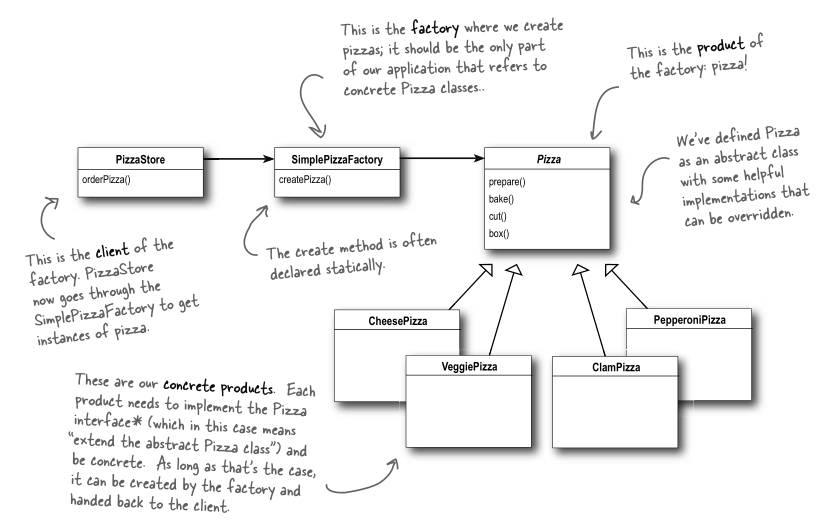
\includegraphics[width=\linewidth]{factory/img/simpleFactoryUML}
	\caption{UML-Darstellung des \emph{einfachen} Factory-Musters}
	\label{fig:simpleFactoryUML}
\end{figure}


\end{document}